
\documentclass{abgabe}

\usepackage{listings}
\usepackage{xcolor}
\usepackage{newtxtt}

\definecolor{darkviolet}{rgb}{0.5,0,0.4}
\definecolor{darkgreen}{rgb}{0,0.4,0.2}
\definecolor{darkblue}{rgb}{0.1,0.1,0.9}
\definecolor{darkgrey}{rgb}{0.5,0.5,0.5}
\definecolor{lightblue}{rgb}{0.4,0.4,1}

\lstset{
    language=Java,
    basicstyle=\small\ttfamily,
    keywordstyle=\color{darkviolet}\bfseries,
    commentstyle=\color{darkgreen},
    stringstyle=\color{darkblue},
    morecomment=[s][\color{lightblue}]{/**}{*/},
    showstringspaces=false,
    frame = single,
    %numbers=left
    }
    
\begin{document}
\begin{questions}
    \qformat{\thequestion. \textbf{\thequestiontitle} \hfill}
    \titledquestion{Politiker}

    Mit dem folgenden Zustandsdiagramm wird das Verhalten eines fiktiven Politikers beschrieben.
    Beachten Sie, dass es eine Parallelkomposition und mehrere hierarchische Zustände gibt.

    Eine Kantenbeschriftung \texttt{e/a} bedeutet, dass nach Erhalt des Ereignisses \texttt{e} eine Aktion \texttt{a} (hier ein internes Ereignis) ausgelöst wird.
    Weiterhin stellen wir Ihnen ein Programmfragment zur Verfügung, mit dem der Nutzer ein solches Objekt steuern kann.
    Die Grundidee ist dabei, dass der Nutzer eine Eingabe macht und das Objekt genau seinen aktuellen Zustand ausgibt.
    Der bereits implementierte Dialog in der hier zur Verfügung gestellten Klasse \texttt{Steuerung}, die noch ergänzt werden muss, hat folgendes Aussehen:

    \begin{lstlisting}
Welches naechste Ereignis?
(0) Lob von der eigenen Partei
(1) Tadel von der eigenen Partei
(2) Lob von der Wirtschaft
(3) Erwischt
1
Fiktiver Politiker befindet sich in (Teil)-Zustaenden:
POLITISCH_AKTIV REBELLISCH PROTEGIERT ERGEBEN
    \end{lstlisting}

    Man sieht die Ausgabe, nachdem der Nutzer das Ereignis \texttt{parteitadel} ausgelöst hat und die genauen Informationen über den aktuellen Zustand ausgegeben werden.

    \newpage

    \begin{lstlisting}[
        language=Java, 
        caption=\texttt{Steuerung.java}, 
        captionpos=b
        ]
import java.util.Scanner;

public class Steuerung {
    private Context_Politiker politiker;	
    
    public Steuerung(){
        int eingabe=-1;
        politiker=new Context_Politiker();
        while(politiker.aktiv()){
            System.out.println("Welches naechste Ereignis?\n"
                    +" (0) Lob von der eigenen Partei\n"
                    +" (1) Tadel von der eigenen Partei\n"
                    +" (2) Lob von der Wirtschaft\n"
                    +" (3) Erwischt");
            eingabe=new Scanner(System.in).nextInt();
            switch(eingabe){
            case 0: 
                politiker.parteilob();
                break;
            case 1:
                politiker.parteitadel();
                break;
            case 2:
                politiker.wirtschaftslob();
                break;
            case 3:
                politiker.erwischt();
                break;
            }
            System.out.println("Fiktiver Politiker befindet sich in"
                    +" (Teil)-Zustaenden: " + politiker);
        }
    }
    
    public static void main(String[] args) {
        new Steuerung();
    }
}
    \end{lstlisting}


    Dieser Zustandsautomat zeigt alle möglichen Zustände und Unterzustände eines Politikers sowie deren Übergänge.

    \begin{center}
        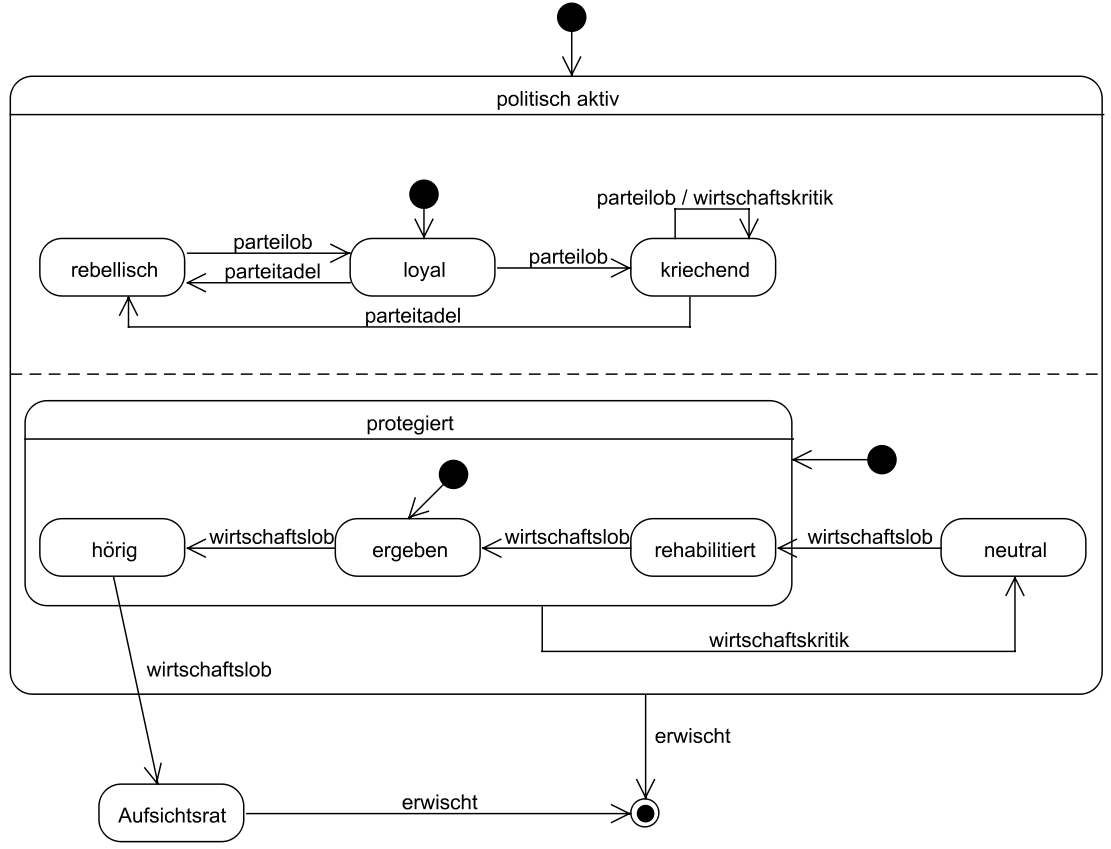
\includegraphics[width=.7\textwidth]{politiker_zustandsautomat.png}
    \end{center}

    \emph{Hinweis:} Dem Endzustand können Sie z.B. den Namen Ruhestand oder Ende geben (in der Implementierung und ggf. bei Aufgabenteil (a).

    \begin{parts}
        \part
        Welchen Zustand erreicht der Automat, nachdem die folgenden Ereignisse aufgetreten sind? (getrennt betrachten)
        \begin{subparts}
            \subpart
            \texttt{parteilob.parteitadel}

            \begin{solution}
                \texttt{POLITISCH\_AKTIV REBELLISCH PROTEGIERT ERGEBEN}
            \end{solution}

            \subpart
            \texttt{parteilob.wirtschaftslob.wirtschaftslob}

            \begin{solution}
                \texttt{POLITISCH\_AKTIV KRIECHEND AUFSICHTSRAT}
            \end{solution}

            \subpart
            \texttt{parteilob.witschaftslob.parteilob.wirtschaftslob}

            \begin{solution}
                \texttt{POLITISCH\_AKTIV KRIECHEND PROTEGIERT REHABILITIERT}
            \end{solution}

            \subpart
            \texttt{parteilob.witschaftslob.erwischt}

            \begin{solution}
                \texttt{RUHESTAND}
            \end{solution}

        \end{subparts}

        \part
        Ihre Aufgabe besteht darin, den Zustandsautomaten präzise unter Nutzung und Ergänzung der Klasse \texttt{Steuerung} (Quellcode siehe oben) zu \emph{implementieren}.

        \emph{Recherchieren Sie das State-Pattern} und setzen Sie den obigen Zustandsautomaten damit um.
        Bedenken Sie dabei, dass ein konkreter Zustand durchaus auch der Context für weitere Unterzustände sein kann.
        Erzeugen Sie im Anschluss an die Implementierung mit Hilfe von Visual Paradigm ein \emph{Klassendiagramm} aus ihrem Code (Sie können natürlich auch mit dem Klassendiagramm beginnen und daraus Code erzeugen!).
        Überprüfen Sie mit Ihrem Code Ihre Ergebnisse aus Aufgabenteil (a).

        Weitere Informationen zur \emph{Code Generation} mit Visual Paradigm finden Sie \href{https://www.visual-paradigm.com/support/documents/vpuserguide/276/381/7486_generateorup.html}{hier}.

        \begin{solution}
            \begin{center}
                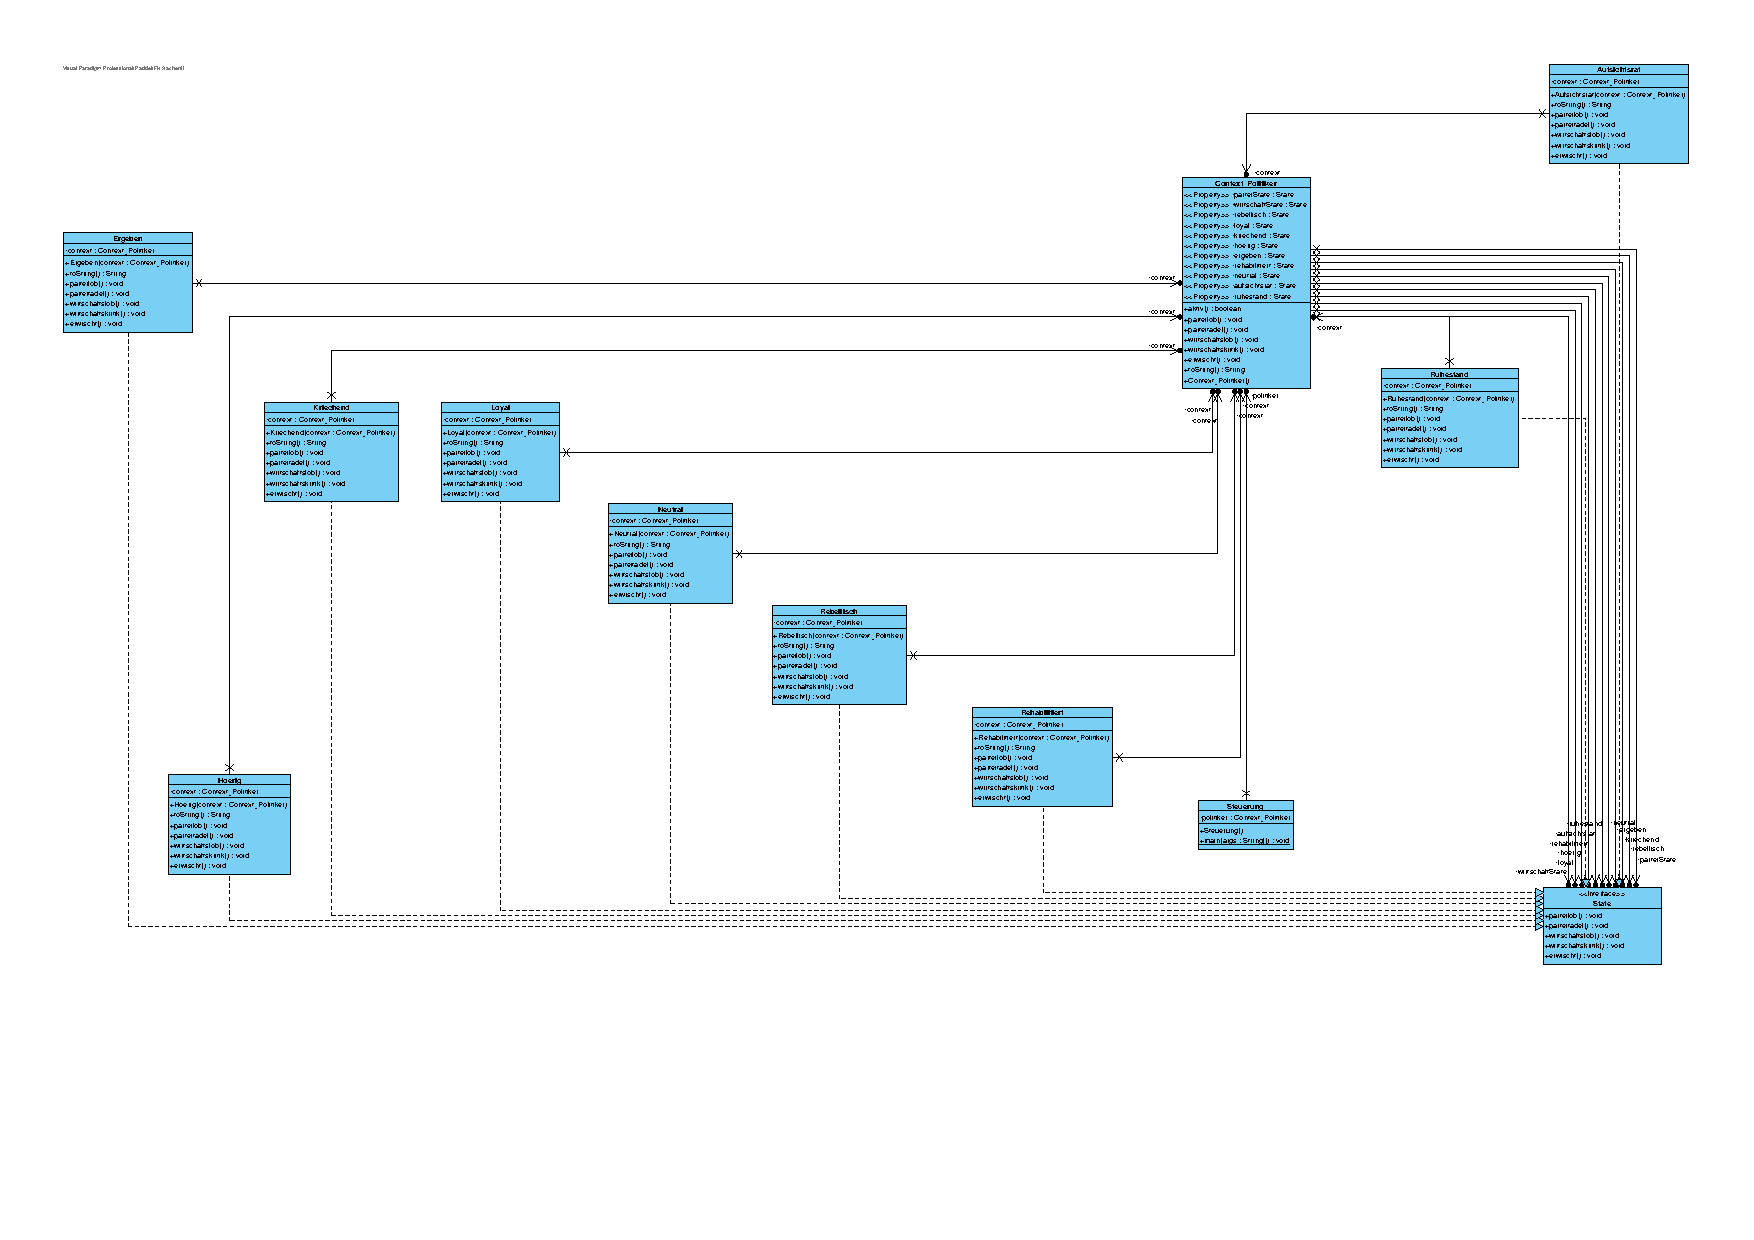
\includegraphics[width=\textwidth]{swt_h10_politiker.pdf}
            \end{center}

            Der Code befindet sich im Anhang.
        \end{solution}
    \end{parts}

    Eine gute Erklärung zum State-Pattern ist \href{https://www.philipphauer.de/study/se/design-pattern/state.php}{hier} zu finden.

    P.S. Machen Sie sich Gedanken darüber, wie eine Aktion wie z.B. \texttt{wirtschaftskritik} aus dem Unterzustand \texttt{politisch aktiv} an \texttt{protegiert} weitergeleitet werden kann.
\end{questions}

\end{document}